%% sample file for Modelica 2021 Conference paper
%% Copyright  Modelica Association
%
% This work may be distributed and/or modified under the
% conditions of the LaTeX Project Public License, either version 1.3
% of this license or (at your option) any later version.
% The latest version of this license is in
%   http://www.latex-project.org/lppl.txt
% and version 1.3 or later is part of all distributions of LaTeX
% version 2005/12/01 or later.
%
% This work is 'maintained' on GitHub:
%   https://github.com/modelica-association/conference-templates
%
% The Current Maintainers are: @akloeckner, @dietmarw, @bernhard-thiele
% With additions by @casella, @sjoelund
%
% This work consists of all files in the GitHub repository except
% a) The files indicated by .gitignore files
% b) The GitHub management files .gitignore, *.md
%
% This class is created from the template for the Modelica 2021 conference

%%% Use the more modern biber and biblatex for Unicode and @online support
\documentclass{modelica}
\addbibresource{modelica2021_ExternData.bib}
\usepackage[utf8]{inputenc} % utf8 input encoding which should work with pdflatex, but not lualatex
\usepackage{cleveref}
% \usepackage[squaren,thinqspace]{SIunits}
% \usepackage{url}
\usepackage{relsize}
% \usepackage{pgfplots}
% \pdfminorversion=4

\hypersetup{%
  pdftitle  = {Efficient Parameterization of Modelica Models},
  pdfauthor = {Thomas Beutlich, Dietmar Winkler},
  pdfsubject = {14th International Modelica Conference 2021},
  pdfkeywords = {Modelica, conference, LaTeX, template},
  colorlinks,
  linkcolor=black,
  urlcolor=black,
  citecolor=black,
  pdfpagelayout = SinglePage,
  pdfcreator = pdflatex,
  pdfproducer = pdflatex}

\lstset{language = c,
       % basicstyle=\fontsize{9pt}{10.5pt}\selectfont,
       basicstyle=\fontsize{9pt}{10.5pt}\ttfamily,
       backgroundcolor = \color{white}}

%c from texinfo.tex
\def\ifmonospace{\ifdim\fontdimen3\font=0pt }

%c C plus plus
\def\C++{%
\ifmonospace%
    C++%
\else%
    C\kern-.1667em\raise.30ex\hbox{\smaller{++}}%
\fi%
\spacefactor1000 }

%c C sharp
\def\Csharp{%
\ifmonospace%
    C\#%
\else%
    C\kern-.1667em\raise.30ex\hbox{\smaller{\#}}%
\fi%
\spacefactor1000 }

\newcommand{\clang}[1]{\lstinline[language=c]|#1|}
\newcommand{\modelica}[1]{\lstinline[language=modelica]|#1|}

\crefformat{footnote}{#2\footnotemark[#1]#3}

% begin the document
\begin{document}
\thispagestyle{empty}

\title{Efficient Parameterization of Modelica Models}
\author[1]{Thomas Beutlich}
\author[2]{Dietmar Winkler}
\affil[1]{Germany, {\small\texttt{modelica@tbeu.de}}}
\affil[2]{University of South-Eastern Norway, {\small\texttt{dietmar.winkler@usn.no}}}

\maketitle\thispagestyle{empty} %% <-- you need this for the first page
\abstract{%
This article explicates the different approaches and use cases for efficient parameterization of Modelica models by means of external data resources.
The main motivation is to improve the overall quality, testability and reusability of Modelica application models (both on component and system level) by a separation of the behavioral implementation from its actual design parameters.
The Modelica libraries \modelica{ExternData} and \modelica{ModelicaTableAdditions} are freely available to support library developers and vendors in their ambitions to offer clean and dedicated interfaces for the parameterization of the application models and to benefit from a large variability of commonly used file types, such as CSV, Excel, HDF, JSON, MATLAB MAT, XML or even domain-specific file types such as for tire properties or weather data.
}

\noindent\emph{Keywords: parameterization, external data resources, Modelica external function interface, SSP}

\section{Introduction}

The separation of the design parameters from Modelica application models was already discussed within the MA (Modelica Association)\footnote{Modelica Association, \url{https://modelica.org}} about 15 years ago.
\textcite{modelica2005Ford} developed an in-house library \modelica{DataRetrieval}, that featured a generic approach applicable for different file formats or data bases.
Supported file formats included for example XML (eXtensible Markup Language), HDF (Hierarchical Data Format) and MATLAB MAT.
There even have been early ideas for the standardization of the appropriate interfaces and XPath query expressions.
Similarly, \textcite{modelica2005ZF} presented an in-house library \modelica{ZFlib} based on simple ASCII text files for a generic parameterization of transmission models.
This library was later extended by \textcite{modelica2006ZF} to also support target platforms without a file system.
\textcite{Reisenbichler2006IfWO} bewailed that the XML technology had not yet established as a standardized concept for the parameterization of Modelica application models.
They again proposed to use XML as file format for external data resources -- being a standardized and widely accepted language with significant tool support for data processing.
Their Dymola\footnote{Dassault Systèmes, \url{https://www.3ds.com}} library also featured the full power of the XPath query expressions and data processing capabilities.

The topic was raised again for the MSL (Modelica Standard Library)\footnote{MA project ``Libraries'', \url{https://doc.modelica.org}} without greater reception in 2008\footnote{MSL issue \#115, \url{https://github.com/modelica/ModelicaStandardLibrary/issues/115}}. Therein it was mentioned, that with the current concept of implementing the data access by the Modelica external function interface, the library vendors and users are responsible to instrument the Modelica code to consider parameterization (described as \emph{pull}-principle). However, with a \emph{push}-principle this responsibility could be moved to the tool vendors, and as such library users could benefit from a greater reusability and flexibility of the layered parameterization.

When the MA project SSP (System Structure and Parameterization of Components for Virtual System Design)\footnote{MA project ``System Structure and Parameterization'', \url{https://ssp-standard.org}} was initiated in 2014, only the parameterization of networks of FMUs (Functional Mock-up Units)\footnote{MA project ``Functional Mock-up Interface'', \url{https://fmi-standard.org}} was considered. Even though the SSP standard 1.0 misses support for array parameters, it was not yet contemplated to apply it as layered standard for the parameterization of Modelica models.

With no standardized interface available, Modelica users depending on external data resources either still need to write their own utility libraries or have to depend on proprietary, tool-specific features (e.g., the data base interface of SimulationX\footnote{SimulationX by ESI,
\url{https://www.simulationx.com}}) or commercially available libraries such as \modelica{Modelon.DataAccess} from Modelon\footnote{Modelon, \url{https://www.modelon.com}}.

\medskip

The parameterization of Modelica models can be differentiated by the following usage scenarios.
\begin{itemize}
 \item Property parameters are constant during a transient simulation. They are non-structural parameters, i.e., a translated simulation model can be reused with changed parameters. Examples are geometry dimensions (e.g., tire diameter), material constants (e.g., electrical resistance) or ambient conditions (e.g., ambient pressure or gravitational acceleration). They can be of \modelica{Real}, \modelica{Integer}, \modelica{Boolean} or \modelica{String} type and either be scalar or of one/two-dimensional array kind (e.g., consumption map or road excitation map).
 \item Stimulation parameters can be considered as time-driven inputs for a transient simulation and can be modeled by one-dimensional look-up tables. Examples are the environmental conditions such as weather.
 \item Structural parameters have influence on the overall system topology and thus on the dimension of the system of equations. They need to be constant during a transient simulation, but any change requires a new translation of the Modelica model. Special care needs to be taken if structural parameters are read from external data resources.
\end{itemize}

The Modelica libraries \modelica{ExternData}\footnote{ExternData Git repository, \url{https://github.com/modelica-3rdparty/ExternData}} and \modelica{ModelicaTableAdditions}\footnote{ModelicaTableAdditions Git repository, \url{https://github.com/tbeu/ModelicaTableAdditions}} are available as open-source Modelica packages under the permissive BSD-2-Clause License.
Both libraries can be directly obtained from GitHub or via the Modelica \modelica{impact} package manager~\cite{impact, Tiller2015WhereIG}.
\begin{itemize}
 \item \modelica{ExternData} supports the user in reading properties or structural parameters from various file types of external data resources.
 Data access from CSV (Comma Separated Values), INI, JSON (JavaScript Object Notation), MATLAB MAT (including HDF), SSV (System Structure Parameter Values), TIR (Tire Properties), Excel XLS/XLSX and XML files is implemented.
 \item \modelica{ModelicaTableAdditions} is an extension of the Modelica Standard Tables~\cite{modelica2014tables} with support for more file types beside Dymola MOS\footnote{There is no specific name or file extension for the Dymola-specific text/script files starting with ``\#1'' as first line.} and MATLAB MAT.
 Its blocks can be utilized to also model stimulation parameterization or look-up tables from CSV, EPW (EnergyPlus Weather)\footnote{EnergyPlus Weather Data, \url{https://energyplus.net/weather}} or JSON files and work as a replacement of the Modelica Standard Tables of the MSL.
\end{itemize}

\section{ExternData}

The Modelica library \modelica{ExternData} developed out of the need to offer an open-source utility package for efficient parameterization of property parameters from external data resources.
It has been successfully tested in Dymola, OpenModelica\footnote{Open Source Modelica Consortium (OSMC),
\url{https://openmodelica.org/}} (Linux only) and SimulationX.

\subsection{Library Design}

The library (as shown in Figure~\ref{fig:ExternData}) consists of top-level data source records for each supported file type, the provided accessor functions in \modelica{ExternData.Functions} and the external objects in \modelica{ExternData.Types}.
\begin{figure}[!hb]
\centering
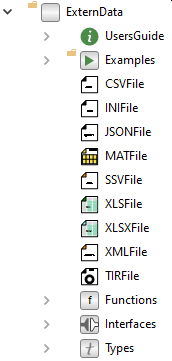
\includegraphics[scale=0.8]{resources/ExternData.png}
\caption{Library structure of \modelica{ExternData}}
\label{fig:ExternData}
\end{figure}

\subsubsection{Data Source Records}

The data source records are convenience types to encapsulate the external object component with its accessor functions.

\begin{lstlisting}[caption=Naive record type definition, label=lst:naive-record-type-definition, language=modelica]
// Library
record DataSource "Data source record"
  parameter String fileName = ""
    "External data resource";
  final parameter Types.ExtObj obj =
    Types.ExtObj(fileName) "Ext. object";
  pure function f "Accessor function"
    input Types.ExtObj obj "Ext. object";
    input String s "Accessor id";
    output Real out "Data value";
    external "C" out = ExtFun(obj, s);
  end f;
end DataSource;

// Application model
parameter DataSource dataSource(
  fileName="dataSource.ext");
parameter Real p = dataSource.f(
  dataSource.obj, "id");
\end{lstlisting}

A naive record type definition together with an exemplary user call (application model) is given in~\autoref{lst:naive-record-type-definition}.
(For the sake of clarity, the declaration of the external type \modelica{Types.ExtObj} and the external function annotation for \modelica{ExtFun} are skipped.)

The disadvantage of such a naive approach is that the handle of the external object, i.e. \modelica{dataSource.obj}, has to be passed by every call of the accessor functions though it actually is an implementation detail of the record and should be a protected component.
A more sophisticated library design is based on clean interfaces for the records and accessor functions enabling inheritance, and thus the possibility of function redeclaration~\cite{modelisax2018hints}.
The general concept is presented in~\autoref{lst:soph-record-type-definition}.

\begin{lstlisting}[caption=Sophisticated record type definition, label=lst:soph-record-type-definition, language=modelica]
// Library
package Interfaces "Interfaces"
  partial record RBase "Base record"
    replaceable function f = fBase;
  end RBase;
  partial function fBase "Base function"
    input Types.ExtObj obj "Ext. object";
    input String s "Accessor id";
    output Real out "Data value";
  end fBase;
end Interfaces;

package Functions "Functions"
  pure function f "Accessor function"
    extends Interfaces.fBase;
    external "C" out = ExtFun(obj, s);
  end f;
end Functions;

record DataSource "Data source record"
  parameter String fileName = ""
    "External data resource";
  final parameter Types.ExtObj obj =
    Types.ExtObj(fileName) "Ext. object";
  extends Interfaces.RBase(
    redeclare final function f =
      Functions.f(obj=obj)
      "Accessor function");
end DataSource;

// Application model
parameter DataSource dataSource(
  fileName="dataSource.ext");
parameter Real p = dataSource.f("id");
\end{lstlisting}

With such a sophisticated library design the actual implementation (as external object) is disguised from the caller as the handle of the external object no longer needs to be passed by the member accessor functions, and hence could be made a protected component.

As of MLS 3.5 (Modelica Language Specification)\footnote{MA project ``Libraries'', \url{https://specification.modelica.org/}}, it is not yet fully specified, if external objects may be used in records\footnote{MLS issue \#2399, \url{https://github.com/modelica/ModelicaSpecification/issues/2399}}.

\subsubsection{External Functions}\label{sec:functions}

The actual external functions and objects serving the Modelica external function interface are implemented in C, i.e. no \C++ is utilized.

Independent of the actual file type, the accessor functions for \modelica{Real}, \modelica{Integer}, \modelica{Boolean} or \modelica{String} scalars are \modelica{getReal}, \modelica{getInteger}, \modelica{getBoolean} or \modelica{getString}, respectively.
For one/two-dimensional arrays, the accessor functions are appended by \modelica{Array1D}/\modelica{Array2D}, e.g., \modelica{getRealArray1D} or \modelica{getIntegerArray2D}.
There also are the corresponding functions to retrieve the array dimensions from the external data resource, i.e., \modelica{getArraySize1D} and \modelica{getArraySize2D} (and also \modelica{getArrayRows2D} and \modelica{getArrayColumns2D}).

\subsubsection{Structural Parameters}

Reading structural parameters using the \modelica{getArraySize1D}/\modelica{getArraySize2D} functions from external data resources (as shown for an XML file by~\autoref{lst:struct-params}) is not generally supported\footnote{MLS issue \#2425, \url{https://github.com/modelica/ModelicaSpecification/issues/2425}}.
Of the tested Modelica tools, it only works in SimulationX.

\begin{lstlisting}[caption=Accessing structural parameters in SimulationX, label=lst:struct-params, language=modelica]
// SimulationX application model
parameter String s = "vector"
  "XML element name";
parameter ExternData.XMLFile dataSource(
  fileName="dataSource.xml")
  "Data source record";
parameter Integer m =
  dataSource.getArraySize1D(s)
  "Structural parameter";
parameter Real p[:] =
  dataSource.getRealArray1D(s, m)
  "Array parameter";
\end{lstlisting}

To assist the Dymola users, alternative implementations using \modelica{readArraySize1D}/\modelica{readArraySize2D} functions are available.
This comes with the disadvantage of redundant file I/O and is demonstrated by~\autoref{lst:struct-params-alt}.

\begin{lstlisting}[caption=Accessing structural parameters in Dymola, label=lst:struct-params-alt, language=modelica]
// Dymola application model
parameter String s = "vector"
  "XML element name";
parameter XMLFile dataSource(
  fileName="dataSource.xml")
  "Data source record";
parameter Integer m =
  ExternData.XMLFile.Functions.
    readArraySize1D(
    varName=s,
    fileName="dataSource.xml")
  "Structural parameter";
parameter Real p[:] =
  dataSource.getRealArray1D(s, m)
  "Array parameter";
\end{lstlisting}

\subsubsection{Missing Data}

In some cases it may happen, that data of the external resources is missing, for example, an empty cell of an Excel file.
By parameter \modelica{detectMissingData}, \modelica{ExternData} supports four options how to deal with missing data values.

\begin{itemize}
 \item Return data-type specific defaults
 \item Return data-type specific defaults and print a message
 \item Return data-type specific defaults and raise a warning
 \item Stop the simulation with an error message
\end{itemize}

Similarly, the accessor functions~(Section \ref{sec:functions}) also return a Boolean output \modelica{exist} to indicate if the retrieved data is available or missing.
This way, the reaction on missing data can be modeled per function call.

\subsection{Supported File Types}

\modelica{ExternData} supports various file types for different kind of requirements.

\subsubsection*{CSV}

CSV files contain exactly one data set that is suitable for one/two-dimensional look-up tables.
An example file with three columns is given by~\autoref{lst:csv-example}.
Both the number of header lines and the column delimiter character can be specified.

\begin{lstlisting}[caption=Example CSV file, label=lst:csv-example]
x,y,z
0,0,0
0.5,0.25,0.125
1,2,3
\end{lstlisting}

\subsubsection*{INI}

INI files contain scalar properties as key-value-pairs which are grouped by sections.
The INI-keys can be fully qualified Modelica names using the dot notation.
An example file with the default section and a named section is given by~\autoref{lst:ini-example}.

\begin{lstlisting}[caption=Example INI file, label=lst:ini-example]
# Default section
gain.k = 1
[Data set]
gain.k = 2
\end{lstlisting}

\subsubsection*{JSON}

JSON files can be used to define scalars, vectors or matrices which can be arbitrarily structured.
The JSON-keys must not contain the dot character to properly work with the accessor functions of \modelica{ExternData}.
An example file with three different values is given by~\autoref{lst:json-example}.

\begin{lstlisting}[caption=Example JSON file, label=lst:json-example]
{
  "Data set": {
    "gain": {
      "k": "2"
    }
  },
  "vector": [1,2,3],
  "matrix": [[0,0],[0.5,0.25],[1,2]]
}
\end{lstlisting}

\subsubsection*{MATLAB MAT (including HDF)}

MATLAB MAT files are binary files that can be used for scalars, vectors or matrices.
Nested structures are possible and can be accessed by \modelica{ExternData} using dot notation.
MATLAB MAT of version~7.3 are HDF5 files and can be considered as a dedicated HDF5 data container.

\subsubsection*{SSV}

SSV files are standardized XML files that are used within the context of SSP to connect and parameterize FMUs.
Certainly, they can not only be used to parameterize imported FMUs in the Modelica simulation environment.
One SSV file describes exactly one parameter set where (as of version~1.0) only scalar parameter values are supported.
\autoref{lst:ssv-example} displays an example SSV file.

\begin{lstlisting}[caption=Example SSV file, label=lst:ssv-example]
<?xml version="1.0" encoding="UTF-8"?>
<ssv:ParameterSet version="1.0" name="Data
  set" xmlns:ssv="http://ssp-standard.org/
  SSP1/SystemStructureParameterValues">
  <ssv:Parameters>
    <ssv:Parameter name="gain.k">
      <ssv:Real value="2"/>
    </ssv:Parameter>
  </ssv:Parameters>
</ssv:ParameterSet>
\end{lstlisting}

Technically, the external object \modelica{ExternData.Types.ExternXML2File} is reused while the SSV accessor functions call the appropriate XML2 functions (\modelica{ExternData.Functions.XML2.*}) with dedicated XPath query expressions.

\subsubsection*{TIR}

TIR files define domain-specific tire properties.
They are similar to INI files and are implemented to share the same external object \modelica{ExternData.Types.ExternINIFile} with respective format permissions.

\subsubsection*{Excel XLS/XLSX}

Both legacy XLS and Office Open XML based XLSX Excel files are supported for parameterization of scalars or matrices.

\subsubsection*{XML}

There are two implementations available.
\begin{enumerate}
 \item \modelica{ExternData.XMLFile} is a straightforward implementation to return values from XML element nodes
 \item \modelica{ExternData.XML2File} enables full support of XPath query expressions to also query XML attributes or more complicated XML structures.
\end{enumerate}

There is no restriction on the underlying XML schema, i.e. it can be used for arbitrarily structured XML data, being standardized (e.g., SSV or CPACS (Common Parametric Aircraft Configuration Schema)\footnote{CPACS, \url{https://cpacs.de}}) or not.

\section{ModelicaTableAdditions}

The Modelica library \modelica{ModelicaTableAdditions} developed out of the need to offer reading of external data sources for stimulation parameters (e.g., look-up tables) from commonly used text file formats.
The Dymola MOS file format, which is the only text file format supported by the Modelica Standard Tables is not suitable for exchange between different applications.
This is where CSV and JSON have their advantages, which can easily be processed by different applications.
As with the Modelica Standard Tables, the external functions are implemented in pure C (i.e., no \C++).
For JSON, the same library dependencies are utilized as with \modelica{ExternData}.
It is possible to use components of packages \modelica{ExternData}, \modelica{ModelicaTableAdditions} and MSL in the same application model.
The library has been successfully tested in Dymola and OpenModelica (Linux only).

\subsection{Library Design}

The library (as shown in Figure~\ref{fig:ModelicaTableAdditions}) consists of the five combi-table blocks known from the MSL, but this time within the \modelica{ModelicaTableAdditions} name-space.

\begin{figure}[!ht]
\centering
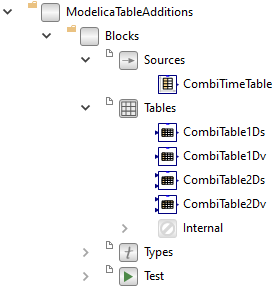
\includegraphics[scale=0.8]{resources/ModelicaTableAdditions.png}
\caption{Library structure of \modelica{ModelicaTableAdditions}}
\label{fig:ModelicaTableAdditions}
\end{figure}

\subsection{Supported File Types}

\subsubsection{CSV}

The table of a CSV file (as shown by~\autoref{lst:csv-example}) can be used for time-driven simulation or one/two-dimensional look-up tables.
Both the number of header lines and the column delimiter character can be specified.

\subsubsection{EPW}

The weather conditions of one year are the typical stimulation parameters for building energy simulations, such as the Modelica \modelica{Buildings} Library~\cite{buildings}.
EnergyPlus provides weather data for simulation in various formats, especially their EPW format.
Since this file format is not natively supported by the Modelica Standard Tables it manually needed to be pre-processed and converted to either Dymola~MOS or MATLAB MAT format.
This pre-processing no longer is necessary as the EPW format is directly supported by all blocks of the \modelica{ModelicaTableAdditions} library.

\subsubsection{JSON}

Similar as with CSV, tables can be read from JSON files and be utilized as stimulation parameters, e.g. parameter ``matrix'' of~\autoref{lst:json-example}.

\section{Conclusions and Outlook}

The open-source libraries \modelica{ExternData} and \modelica{ModelicaTableAdditions} are an offer to Modelica library developers and users to efficiently parameterize Modelica application models.
Its right to exist is due to a missing layered (MA) standard for the parameterization of Modelica models.
As already mentioned by~\textcite{modelica2005Ford}, the benefits of such a standardization are the cutback of library code towards the Modelica tools to even further increase the efficiency, convenience and usability of the parameterization of application models.

There is no support for units so far, i.e., unit conversion is left to the application.
This could be also addressed by a standardized parameterization.

Library-wise, one future idea is the support of (symmetrical of asymmetrical) encrypted external resources, which is not yet covered by the MLS.
In such cases the external functions require the appropriate (private) key to decrypt the external resources at simulation run-time in memory.
Again, encryption as an isolated application can only be considered a short-term solution towards a future standard.

Furthermore, it might be desirable if the mentioned open issues on the MLS regarding external objects could be clarified finally.

\section*{Acknowledgements}

The authors would like to thank everybody who has contributed to the libraries \modelica{ExternData} and \modelica{ModelicaTableAdditions}, particularly, Hang Yu, Martin Sjölund, Mike Dempsey and Peter Harman.

\printbibliography

\end{document}
